\documentclass[11pt]{article}
\usepackage{sectsty}
\allsectionsfont{\color{blue}\fontfamily{lmss}\selectfont}
\usepackage{fontspec}
\setmainfont{XCharter}

\usepackage{listings}
\lstset{
basicstyle=\small\ttfamily,
tabsize=8,
columns=flexible,
breaklines=true,
frame=tb,
rulecolor=\color[rgb]{0.8,0.8,0.7},
backgroundcolor=\color[rgb]{1,1,0.91},
postbreak=\raisebox{0ex}[0ex][0ex]{\ensuremath{\color{red}\hookrightarrow\space}}
}
\usepackage{fontawesome}


\usepackage{mdframed}
\newmdenv[
  backgroundcolor=gray,
  fontcolor=white,
  nobreak=true,
]{terminalinput}



\usepackage{parskip}


    \usepackage[breakable]{tcolorbox}
    \usepackage{parskip} % Stop auto-indenting (to mimic markdown behaviour)


    % Basic figure setup, for now with no caption control since it's done
    % automatically by Pandoc (which extracts ![](path) syntax from Markdown).
    \usepackage{graphicx}
    % Maintain compatibility with old templates. Remove in nbconvert 6.0
    \let\Oldincludegraphics\includegraphics
    % Ensure that by default, figures have no caption (until we provide a
    % proper Figure object with a Caption API and a way to capture that
    % in the conversion process - todo).
    \usepackage{caption}
    \DeclareCaptionFormat{nocaption}{}
    \captionsetup{format=nocaption,aboveskip=0pt,belowskip=0pt}

    \usepackage{float}
    \floatplacement{figure}{H} % forces figures to be placed at the correct location
    \usepackage{xcolor} % Allow colors to be defined
    \usepackage{enumerate} % Needed for markdown enumerations to work
    \usepackage{geometry} % Used to adjust the document margins
    \usepackage{amsmath} % Equations
    \usepackage{amssymb} % Equations
    \usepackage{textcomp} % defines textquotesingle
    % Hack from http://tex.stackexchange.com/a/47451/13684:
    \AtBeginDocument{%
        \def\PYZsq{\textquotesingle}% Upright quotes in Pygmentized code
    }
    \usepackage{upquote} % Upright quotes for verbatim code
    \usepackage{eurosym} % defines \euro

    \usepackage{iftex}
    \ifPDFTeX
        \usepackage[T1]{fontenc}
        \IfFileExists{alphabeta.sty}{
              \usepackage{alphabeta}
          }{
              \usepackage[mathletters]{ucs}
              \usepackage[utf8x]{inputenc}
          }
    \else
        \usepackage{fontspec}
        \usepackage{unicode-math}
    \fi

    \usepackage{fancyvrb} % verbatim replacement that allows latex
    \usepackage{grffile} % extends the file name processing of package graphics
                         % to support a larger range
    \makeatletter % fix for old versions of grffile with XeLaTeX
    \@ifpackagelater{grffile}{2019/11/01}
    {
      % Do nothing on new versions
    }
    {
      \def\Gread@@xetex#1{%
        \IfFileExists{"\Gin@base".bb}%
        {\Gread@eps{\Gin@base.bb}}%
        {\Gread@@xetex@aux#1}%
      }
    }
    \makeatother
    \usepackage[Export]{adjustbox} % Used to constrain images to a maximum size
    \adjustboxset{max size={0.9\linewidth}{0.9\paperheight}}

    % The hyperref package gives us a pdf with properly built
    % internal navigation ('pdf bookmarks' for the table of contents,
    % internal cross-reference links, web links for URLs, etc.)
    \usepackage{hyperref}
    % The default LaTeX title has an obnoxious amount of whitespace. By default,
    % titling removes some of it. It also provides customization options.
    \usepackage{titling}
    \usepackage{longtable} % longtable support required by pandoc >1.10
    \usepackage{booktabs}  % table support for pandoc > 1.12.2
    \usepackage{array}     % table support for pandoc >= 2.11.3
    \usepackage{calc}      % table minipage width calculation for pandoc >= 2.11.1
    \usepackage[inline]{enumitem} % IRkernel/repr support (it uses the enumerate* environment)
    \usepackage[normalem]{ulem} % ulem is needed to support strikethroughs (\sout)
                                % normalem makes italics be italics, not underlines
    \usepackage{mathrsfs}



    % Colors for the hyperref package
    \definecolor{urlcolor}{rgb}{0,.145,.698}
    \definecolor{linkcolor}{rgb}{.71,0.21,0.01}
    \definecolor{citecolor}{rgb}{.12,.54,.11}

    % ANSI colors
    \definecolor{ansi-black}{HTML}{3E424D}
    \definecolor{ansi-black-intense}{HTML}{282C36}
    \definecolor{ansi-red}{HTML}{E75C58}
    \definecolor{ansi-red-intense}{HTML}{B22B31}
    \definecolor{ansi-green}{HTML}{00A250}
    \definecolor{ansi-green-intense}{HTML}{007427}
    \definecolor{ansi-yellow}{HTML}{DDB62B}
    \definecolor{ansi-yellow-intense}{HTML}{B27D12}
    \definecolor{ansi-blue}{HTML}{208FFB}
    \definecolor{ansi-blue-intense}{HTML}{0065CA}
    \definecolor{ansi-magenta}{HTML}{D160C4}
    \definecolor{ansi-magenta-intense}{HTML}{A03196}
    \definecolor{ansi-cyan}{HTML}{60C6C8}
    \definecolor{ansi-cyan-intense}{HTML}{258F8F}
    \definecolor{ansi-white}{HTML}{C5C1B4}
    \definecolor{ansi-white-intense}{HTML}{A1A6B2}
    \definecolor{ansi-default-inverse-fg}{HTML}{FFFFFF}
    \definecolor{ansi-default-inverse-bg}{HTML}{000000}

    % common color for the border for error outputs.
    \definecolor{outerrorbackground}{HTML}{FFDFDF}

    % commands and environments needed by pandoc snippets
    % extracted from the output of `pandoc -s`
    \providecommand{\tightlist}{%
      \setlength{\itemsep}{0pt}\setlength{\parskip}{0pt}}
    \DefineVerbatimEnvironment{Highlighting}{Verbatim}{commandchars=\\\{\}}
    % Add ',fontsize=\small' for more characters per line
    \newenvironment{Shaded}{}{}
    \newcommand{\KeywordTok}[1]{\textcolor[rgb]{0.00,0.44,0.13}{\textbf{{#1}}}}
    \newcommand{\DataTypeTok}[1]{\textcolor[rgb]{0.56,0.13,0.00}{{#1}}}
    \newcommand{\DecValTok}[1]{\textcolor[rgb]{0.25,0.63,0.44}{{#1}}}
    \newcommand{\BaseNTok}[1]{\textcolor[rgb]{0.25,0.63,0.44}{{#1}}}
    \newcommand{\FloatTok}[1]{\textcolor[rgb]{0.25,0.63,0.44}{{#1}}}
    \newcommand{\CharTok}[1]{\textcolor[rgb]{0.25,0.44,0.63}{{#1}}}
    \newcommand{\StringTok}[1]{\textcolor[rgb]{0.25,0.44,0.63}{{#1}}}
    \newcommand{\CommentTok}[1]{\textcolor[rgb]{0.38,0.63,0.69}{\textit{{#1}}}}
    \newcommand{\OtherTok}[1]{\textcolor[rgb]{0.00,0.44,0.13}{{#1}}}
    \newcommand{\AlertTok}[1]{\textcolor[rgb]{1.00,0.00,0.00}{\textbf{{#1}}}}
    \newcommand{\FunctionTok}[1]{\textcolor[rgb]{0.02,0.16,0.49}{{#1}}}
    \newcommand{\RegionMarkerTok}[1]{{#1}}
    \newcommand{\ErrorTok}[1]{\textcolor[rgb]{1.00,0.00,0.00}{\textbf{{#1}}}}
    \newcommand{\NormalTok}[1]{{#1}}

    % Additional commands for more recent versions of Pandoc
    \newcommand{\ConstantTok}[1]{\textcolor[rgb]{0.53,0.00,0.00}{{#1}}}
    \newcommand{\SpecialCharTok}[1]{\textcolor[rgb]{0.25,0.44,0.63}{{#1}}}
    \newcommand{\VerbatimStringTok}[1]{\textcolor[rgb]{0.25,0.44,0.63}{{#1}}}
    \newcommand{\SpecialStringTok}[1]{\textcolor[rgb]{0.73,0.40,0.53}{{#1}}}
    \newcommand{\ImportTok}[1]{{#1}}
    \newcommand{\DocumentationTok}[1]{\textcolor[rgb]{0.73,0.13,0.13}{\textit{{#1}}}}
    \newcommand{\AnnotationTok}[1]{\textcolor[rgb]{0.38,0.63,0.69}{\textbf{\textit{{#1}}}}}
    \newcommand{\CommentVarTok}[1]{\textcolor[rgb]{0.38,0.63,0.69}{\textbf{\textit{{#1}}}}}
    \newcommand{\VariableTok}[1]{\textcolor[rgb]{0.10,0.09,0.49}{{#1}}}
    \newcommand{\ControlFlowTok}[1]{\textcolor[rgb]{0.00,0.44,0.13}{\textbf{{#1}}}}
    \newcommand{\OperatorTok}[1]{\textcolor[rgb]{0.40,0.40,0.40}{{#1}}}
    \newcommand{\BuiltInTok}[1]{{#1}}
    \newcommand{\ExtensionTok}[1]{{#1}}
    \newcommand{\PreprocessorTok}[1]{\textcolor[rgb]{0.74,0.48,0.00}{{#1}}}
    \newcommand{\AttributeTok}[1]{\textcolor[rgb]{0.49,0.56,0.16}{{#1}}}
    \newcommand{\InformationTok}[1]{\textcolor[rgb]{0.38,0.63,0.69}{\textbf{\textit{{#1}}}}}
    \newcommand{\WarningTok}[1]{\textcolor[rgb]{0.38,0.63,0.69}{\textbf{\textit{{#1}}}}}


    % Define a nice break command that doesn't care if a line doesn't already
    % exist.
    \def\br{\hspace*{\fill} \\* }
    % Math Jax compatibility definitions
    \def\gt{>}
    \def\lt{<}
    \let\Oldtex\TeX
    \let\Oldlatex\LaTeX
    \renewcommand{\TeX}{\textrm{\Oldtex}}
    \renewcommand{\LaTeX}{\textrm{\Oldlatex}}
    % Document parameters
    % Document title
    \title{project1}







% Pygments definitions
\makeatletter
\def\PY@reset{\let\PY@it=\relax \let\PY@bf=\relax%
    \let\PY@ul=\relax \let\PY@tc=\relax%
    \let\PY@bc=\relax \let\PY@ff=\relax}
\def\PY@tok#1{\csname PY@tok@#1\endcsname}
\def\PY@toks#1+{\ifx\relax#1\empty\else%
    \PY@tok{#1}\expandafter\PY@toks\fi}
\def\PY@do#1{\PY@bc{\PY@tc{\PY@ul{%
    \PY@it{\PY@bf{\PY@ff{#1}}}}}}}
\def\PY#1#2{\PY@reset\PY@toks#1+\relax+\PY@do{#2}}

\@namedef{PY@tok@w}{\def\PY@tc##1{\textcolor[rgb]{0.73,0.73,0.73}{##1}}}
\@namedef{PY@tok@c}{\let\PY@it=\textit\def\PY@tc##1{\textcolor[rgb]{0.24,0.48,0.48}{##1}}}
\@namedef{PY@tok@cp}{\def\PY@tc##1{\textcolor[rgb]{0.61,0.40,0.00}{##1}}}
\@namedef{PY@tok@k}{\let\PY@bf=\textbf\def\PY@tc##1{\textcolor[rgb]{0.00,0.50,0.00}{##1}}}
\@namedef{PY@tok@kp}{\def\PY@tc##1{\textcolor[rgb]{0.00,0.50,0.00}{##1}}}
\@namedef{PY@tok@kt}{\def\PY@tc##1{\textcolor[rgb]{0.69,0.00,0.25}{##1}}}
\@namedef{PY@tok@o}{\def\PY@tc##1{\textcolor[rgb]{0.40,0.40,0.40}{##1}}}
\@namedef{PY@tok@ow}{\let\PY@bf=\textbf\def\PY@tc##1{\textcolor[rgb]{0.67,0.13,1.00}{##1}}}
\@namedef{PY@tok@nb}{\def\PY@tc##1{\textcolor[rgb]{0.00,0.50,0.00}{##1}}}
\@namedef{PY@tok@nf}{\def\PY@tc##1{\textcolor[rgb]{0.00,0.00,1.00}{##1}}}
\@namedef{PY@tok@nc}{\let\PY@bf=\textbf\def\PY@tc##1{\textcolor[rgb]{0.00,0.00,1.00}{##1}}}
\@namedef{PY@tok@nn}{\let\PY@bf=\textbf\def\PY@tc##1{\textcolor[rgb]{0.00,0.00,1.00}{##1}}}
\@namedef{PY@tok@ne}{\let\PY@bf=\textbf\def\PY@tc##1{\textcolor[rgb]{0.80,0.25,0.22}{##1}}}
\@namedef{PY@tok@nv}{\def\PY@tc##1{\textcolor[rgb]{0.10,0.09,0.49}{##1}}}
\@namedef{PY@tok@no}{\def\PY@tc##1{\textcolor[rgb]{0.53,0.00,0.00}{##1}}}
\@namedef{PY@tok@nl}{\def\PY@tc##1{\textcolor[rgb]{0.46,0.46,0.00}{##1}}}
\@namedef{PY@tok@ni}{\let\PY@bf=\textbf\def\PY@tc##1{\textcolor[rgb]{0.44,0.44,0.44}{##1}}}
\@namedef{PY@tok@na}{\def\PY@tc##1{\textcolor[rgb]{0.41,0.47,0.13}{##1}}}
\@namedef{PY@tok@nt}{\let\PY@bf=\textbf\def\PY@tc##1{\textcolor[rgb]{0.00,0.50,0.00}{##1}}}
\@namedef{PY@tok@nd}{\def\PY@tc##1{\textcolor[rgb]{0.67,0.13,1.00}{##1}}}
\@namedef{PY@tok@s}{\def\PY@tc##1{\textcolor[rgb]{0.73,0.13,0.13}{##1}}}
\@namedef{PY@tok@sd}{\let\PY@it=\textit\def\PY@tc##1{\textcolor[rgb]{0.73,0.13,0.13}{##1}}}
\@namedef{PY@tok@si}{\let\PY@bf=\textbf\def\PY@tc##1{\textcolor[rgb]{0.64,0.35,0.47}{##1}}}
\@namedef{PY@tok@se}{\let\PY@bf=\textbf\def\PY@tc##1{\textcolor[rgb]{0.67,0.36,0.12}{##1}}}
\@namedef{PY@tok@sr}{\def\PY@tc##1{\textcolor[rgb]{0.64,0.35,0.47}{##1}}}
\@namedef{PY@tok@ss}{\def\PY@tc##1{\textcolor[rgb]{0.10,0.09,0.49}{##1}}}
\@namedef{PY@tok@sx}{\def\PY@tc##1{\textcolor[rgb]{0.00,0.50,0.00}{##1}}}
\@namedef{PY@tok@m}{\def\PY@tc##1{\textcolor[rgb]{0.40,0.40,0.40}{##1}}}
\@namedef{PY@tok@gh}{\let\PY@bf=\textbf\def\PY@tc##1{\textcolor[rgb]{0.00,0.00,0.50}{##1}}}
\@namedef{PY@tok@gu}{\let\PY@bf=\textbf\def\PY@tc##1{\textcolor[rgb]{0.50,0.00,0.50}{##1}}}
\@namedef{PY@tok@gd}{\def\PY@tc##1{\textcolor[rgb]{0.63,0.00,0.00}{##1}}}
\@namedef{PY@tok@gi}{\def\PY@tc##1{\textcolor[rgb]{0.00,0.52,0.00}{##1}}}
\@namedef{PY@tok@gr}{\def\PY@tc##1{\textcolor[rgb]{0.89,0.00,0.00}{##1}}}
\@namedef{PY@tok@ge}{\let\PY@it=\textit}
\@namedef{PY@tok@gs}{\let\PY@bf=\textbf}
\@namedef{PY@tok@gp}{\let\PY@bf=\textbf\def\PY@tc##1{\textcolor[rgb]{0.00,0.00,0.50}{##1}}}
\@namedef{PY@tok@go}{\def\PY@tc##1{\textcolor[rgb]{0.44,0.44,0.44}{##1}}}
\@namedef{PY@tok@gt}{\def\PY@tc##1{\textcolor[rgb]{0.00,0.27,0.87}{##1}}}
\@namedef{PY@tok@err}{\def\PY@bc##1{{\setlength{\fboxsep}{\string -\fboxrule}\fcolorbox[rgb]{1.00,0.00,0.00}{1,1,1}{\strut ##1}}}}
\@namedef{PY@tok@kc}{\let\PY@bf=\textbf\def\PY@tc##1{\textcolor[rgb]{0.00,0.50,0.00}{##1}}}
\@namedef{PY@tok@kd}{\let\PY@bf=\textbf\def\PY@tc##1{\textcolor[rgb]{0.00,0.50,0.00}{##1}}}
\@namedef{PY@tok@kn}{\let\PY@bf=\textbf\def\PY@tc##1{\textcolor[rgb]{0.00,0.50,0.00}{##1}}}
\@namedef{PY@tok@kr}{\let\PY@bf=\textbf\def\PY@tc##1{\textcolor[rgb]{0.00,0.50,0.00}{##1}}}
\@namedef{PY@tok@bp}{\def\PY@tc##1{\textcolor[rgb]{0.00,0.50,0.00}{##1}}}
\@namedef{PY@tok@fm}{\def\PY@tc##1{\textcolor[rgb]{0.00,0.00,1.00}{##1}}}
\@namedef{PY@tok@vc}{\def\PY@tc##1{\textcolor[rgb]{0.10,0.09,0.49}{##1}}}
\@namedef{PY@tok@vg}{\def\PY@tc##1{\textcolor[rgb]{0.10,0.09,0.49}{##1}}}
\@namedef{PY@tok@vi}{\def\PY@tc##1{\textcolor[rgb]{0.10,0.09,0.49}{##1}}}
\@namedef{PY@tok@vm}{\def\PY@tc##1{\textcolor[rgb]{0.10,0.09,0.49}{##1}}}
\@namedef{PY@tok@sa}{\def\PY@tc##1{\textcolor[rgb]{0.73,0.13,0.13}{##1}}}
\@namedef{PY@tok@sb}{\def\PY@tc##1{\textcolor[rgb]{0.73,0.13,0.13}{##1}}}
\@namedef{PY@tok@sc}{\def\PY@tc##1{\textcolor[rgb]{0.73,0.13,0.13}{##1}}}
\@namedef{PY@tok@dl}{\def\PY@tc##1{\textcolor[rgb]{0.73,0.13,0.13}{##1}}}
\@namedef{PY@tok@s2}{\def\PY@tc##1{\textcolor[rgb]{0.73,0.13,0.13}{##1}}}
\@namedef{PY@tok@sh}{\def\PY@tc##1{\textcolor[rgb]{0.73,0.13,0.13}{##1}}}
\@namedef{PY@tok@s1}{\def\PY@tc##1{\textcolor[rgb]{0.73,0.13,0.13}{##1}}}
\@namedef{PY@tok@mb}{\def\PY@tc##1{\textcolor[rgb]{0.40,0.40,0.40}{##1}}}
\@namedef{PY@tok@mf}{\def\PY@tc##1{\textcolor[rgb]{0.40,0.40,0.40}{##1}}}
\@namedef{PY@tok@mh}{\def\PY@tc##1{\textcolor[rgb]{0.40,0.40,0.40}{##1}}}
\@namedef{PY@tok@mi}{\def\PY@tc##1{\textcolor[rgb]{0.40,0.40,0.40}{##1}}}
\@namedef{PY@tok@il}{\def\PY@tc##1{\textcolor[rgb]{0.40,0.40,0.40}{##1}}}
\@namedef{PY@tok@mo}{\def\PY@tc##1{\textcolor[rgb]{0.40,0.40,0.40}{##1}}}
\@namedef{PY@tok@ch}{\let\PY@it=\textit\def\PY@tc##1{\textcolor[rgb]{0.24,0.48,0.48}{##1}}}
\@namedef{PY@tok@cm}{\let\PY@it=\textit\def\PY@tc##1{\textcolor[rgb]{0.24,0.48,0.48}{##1}}}
\@namedef{PY@tok@cpf}{\let\PY@it=\textit\def\PY@tc##1{\textcolor[rgb]{0.24,0.48,0.48}{##1}}}
\@namedef{PY@tok@c1}{\let\PY@it=\textit\def\PY@tc##1{\textcolor[rgb]{0.24,0.48,0.48}{##1}}}
\@namedef{PY@tok@cs}{\let\PY@it=\textit\def\PY@tc##1{\textcolor[rgb]{0.24,0.48,0.48}{##1}}}

\def\PYZbs{\char`\\}
\def\PYZus{\char`\_}
\def\PYZob{\char`\{}
\def\PYZcb{\char`\}}
\def\PYZca{\char`\^}
\def\PYZam{\char`\&}
\def\PYZlt{\char`\<}
\def\PYZgt{\char`\>}
\def\PYZsh{\char`\#}
\def\PYZpc{\char`\%}
\def\PYZdl{\char`\$}
\def\PYZhy{\char`\-}
\def\PYZsq{\char`\'}
\def\PYZdq{\char`\"}
\def\PYZti{\char`\~}
% for compatibility with earlier versions
\def\PYZat{@}
\def\PYZlb{[}
\def\PYZrb{]}
\makeatother


    % For linebreaks inside Verbatim environment from package fancyvrb.
    \makeatletter
        \newbox\Wrappedcontinuationbox
        \newbox\Wrappedvisiblespacebox
        \newcommand*\Wrappedvisiblespace {\textcolor{red}{\textvisiblespace}}
        \newcommand*\Wrappedcontinuationsymbol {\textcolor{red}{\llap{\tiny$\m@th\hookrightarrow$}}}
        \newcommand*\Wrappedcontinuationindent {3ex }
        \newcommand*\Wrappedafterbreak {\kern\Wrappedcontinuationindent\copy\Wrappedcontinuationbox}
        % Take advantage of the already applied Pygments mark-up to insert
        % potential linebreaks for TeX processing.
        %        {, <, #, %, $, ' and ": go to next line.
        %        _, }, ^, &, >, - and ~: stay at end of broken line.
        % Use of \textquotesingle for straight quote.
        \newcommand*\Wrappedbreaksatspecials {%
            \def\PYGZus{\discretionary{\char`\_}{\Wrappedafterbreak}{\char`\_}}%
            \def\PYGZob{\discretionary{}{\Wrappedafterbreak\char`\{}{\char`\{}}%
            \def\PYGZcb{\discretionary{\char`\}}{\Wrappedafterbreak}{\char`\}}}%
            \def\PYGZca{\discretionary{\char`\^}{\Wrappedafterbreak}{\char`\^}}%
            \def\PYGZam{\discretionary{\char`\&}{\Wrappedafterbreak}{\char`\&}}%
            \def\PYGZlt{\discretionary{}{\Wrappedafterbreak\char`\<}{\char`\<}}%
            \def\PYGZgt{\discretionary{\char`\>}{\Wrappedafterbreak}{\char`\>}}%
            \def\PYGZsh{\discretionary{}{\Wrappedafterbreak\char`\#}{\char`\#}}%
            \def\PYGZpc{\discretionary{}{\Wrappedafterbreak\char`\%}{\char`\%}}%
            \def\PYGZdl{\discretionary{}{\Wrappedafterbreak\char`\$}{\char`\$}}%
            \def\PYGZhy{\discretionary{\char`\-}{\Wrappedafterbreak}{\char`\-}}%
            \def\PYGZsq{\discretionary{}{\Wrappedafterbreak\textquotesingle}{\textquotesingle}}%
            \def\PYGZdq{\discretionary{}{\Wrappedafterbreak\char`\"}{\char`\"}}%
            \def\PYGZti{\discretionary{\char`\~}{\Wrappedafterbreak}{\char`\~}}%
        }
        % Some characters . , ; ? ! / are not pygmentized.
        % This macro makes them "active" and they will insert potential linebreaks
        \newcommand*\Wrappedbreaksatpunct {%
            \lccode`\~`\.\lowercase{\def~}{\discretionary{\hbox{\char`\.}}{\Wrappedafterbreak}{\hbox{\char`\.}}}%
            \lccode`\~`\,\lowercase{\def~}{\discretionary{\hbox{\char`\,}}{\Wrappedafterbreak}{\hbox{\char`\,}}}%
            \lccode`\~`\;\lowercase{\def~}{\discretionary{\hbox{\char`\;}}{\Wrappedafterbreak}{\hbox{\char`\;}}}%
            \lccode`\~`\:\lowercase{\def~}{\discretionary{\hbox{\char`\:}}{\Wrappedafterbreak}{\hbox{\char`\:}}}%
            \lccode`\~`\?\lowercase{\def~}{\discretionary{\hbox{\char`\?}}{\Wrappedafterbreak}{\hbox{\char`\?}}}%
            \lccode`\~`\!\lowercase{\def~}{\discretionary{\hbox{\char`\!}}{\Wrappedafterbreak}{\hbox{\char`\!}}}%
            \lccode`\~`\/\lowercase{\def~}{\discretionary{\hbox{\char`\/}}{\Wrappedafterbreak}{\hbox{\char`\/}}}%
            \catcode`\.\active
            \catcode`\,\active
            \catcode`\;\active
            \catcode`\:\active
            \catcode`\?\active
            \catcode`\!\active
            \catcode`\/\active
            \lccode`\~`\~
        }
    \makeatother

    \let\OriginalVerbatim=\Verbatim
    \makeatletter
    \renewcommand{\Verbatim}[1][1]{%
        %\parskip\z@skip
        \sbox\Wrappedcontinuationbox {\Wrappedcontinuationsymbol}%
        \sbox\Wrappedvisiblespacebox {\FV@SetupFont\Wrappedvisiblespace}%
        \def\FancyVerbFormatLine ##1{\hsize\linewidth
            \vtop{\raggedright\hyphenpenalty\z@\exhyphenpenalty\z@
                \doublehyphendemerits\z@\finalhyphendemerits\z@
                \strut ##1\strut}%
        }%
        % If the linebreak is at a space, the latter will be displayed as visible
        % space at end of first line, and a continuation symbol starts next line.
        % Stretch/shrink are however usually zero for typewriter font.
        \def\FV@Space {%
            \nobreak\hskip\z@ plus\fontdimen3\font minus\fontdimen4\font
            \discretionary{\copy\Wrappedvisiblespacebox}{\Wrappedafterbreak}
            {\kern\fontdimen2\font}%
        }%

        % Allow breaks at special characters using \PYG... macros.
        \Wrappedbreaksatspecials
        % Breaks at punctuation characters . , ; ? ! and / need catcode=\active
        \OriginalVerbatim[#1,codes*=\Wrappedbreaksatpunct]%
    }
    \makeatother

    % Exact colors from NB
    \definecolor{incolor}{HTML}{303F9F}
    \definecolor{outcolor}{HTML}{D84315}
    \definecolor{cellborder}{HTML}{CFCFCF}
    \definecolor{cellbackground}{HTML}{F7F7F7}

    % prompt
    \makeatletter
    \newcommand{\boxspacing}{\kern\kvtcb@left@rule\kern\kvtcb@boxsep}
    \makeatother
    \newcommand{\prompt}[4]{
        {\ttfamily\llap{{\color{#2}[#3]:\hspace{3pt}#4}}\vspace{-\baselineskip}}
    }



    % Prevent overflowing lines due to hard-to-break entities
    \sloppy
    % Setup hyperref package
    \hypersetup{
      breaklinks=true,  % so long urls are correctly broken across lines
      colorlinks=true,
      urlcolor=urlcolor,
      linkcolor=linkcolor,
      citecolor=citecolor,
      }
    % Slightly bigger margins than the latex defaults

    \geometry{verbose,tmargin=1in,bmargin=1in,lmargin=1in,rmargin=1in}



\renewcommand{\PY}[2]{{#2}}
\usepackage{fancyhdr}
\pagestyle{fancy}
\rhead{\color{gray}\sf\small\rightmark}
\lhead{\nouppercase{\color{gray}\sf\small\leftmark}}
\cfoot{\color{gray}\sf\thepage}
\renewcommand{\footrulewidth}{1pt}
\begin{document}





    \hypertarget{genomic-analysis-of-salmonella-typhimurium}{%
\section{Genomic analysis of Salmonella
Typhimurium}\label{genomic-analysis-of-salmonella-typhimurium}}

For this analysis project, you will use the all the skills acquired from
earlier in the week to map the sequnce data of 25 isolates of Salmonella
Typhimurium to the reference sequence strain construct a phylogenetic
tree. You will use the software FigTree to view and interpret your
phylogeny and also use Microreact to visualise location data and develop
your own hypotheses about the pathogen distribution. In addition, you
will use the software ARIBA (Antibiotic Resistance Identification By
Assembly) to investigate resistance genes in these strains and a free
visualisation tool, Phandango to compare with the pathogen distribution
observed in your tree. You will also prepare a short 5 mins presentation
describing the analysis approach and your key findings.

    \hypertarget{learning-outcomes}{%
\section{Learning outcomes:}\label{learning-outcomes}}

On completion of the assignment, you can expect to have acquired the
skills to:

\begin{itemize}
\tightlist
\item
  Build and interpret phylogenetic trees from Whole Genome Sequence
  (WGS) data of bacterial samples
\item
  Show how WGS can be used to describe the evolution and distribution of
  a pathogen across a geographical area
\item
  Combine phylogenetic analysis and AMR results
\item
  Present the results of WGS data analysis
\end{itemize}

    \hypertarget{introducing-the-dataset}{%
\section{Introducing the dataset}\label{introducing-the-dataset}}

Salmonella enterica is a diverse bacterial species that can cause
disease in both human and animals. Human infections caused by Salmonella
can be divided into two, typhoidal Salmonella or non-typhoidal
Salmonella (NTS). The former include Typhi and Paratyphi serovars that
cause typhoid. NTS comprises of multiple serovars that cause
self-limiting gastroenteritis in humans and is normally associated with
zoonotic Salmonella reservoirs, typically domesticated animals, with
little or no sustained human-to-human transmission.

Salmonella enterica serovar Typhimurium (S. Typhimurium), unlike the
classical views of NTS, can cause an invasive form of NTS (iNTS), with
distinct clinical representations to typhoid and gastroenteritis and
normally characterized by a nonspecific fever that can be
indistinguishable from malaria and in rare cases is accompanied by
diarrhoea.

You have been provided with sequence data for 25 S. Typhimurium isolates
collected from regional labs in England and Wales throughout 2022. Whole
genome sequence analysis of this organism can provide some insight into
the short-term microevolution of S. Typhimurium. Understanding the level
of diversity in this time-period is crucial in attempting to identify if
this is an outbreak or sporadic infection.

To download the data that you need for this asignment:

    \begin{tcolorbox}[breakable, size=fbox, boxrule=1pt, pad at break*=1mm,colback=cellbackground, colframe=cellborder]
\prompt{In}{incolor}{ }{\boxspacing}
\begin{Verbatim}[commandchars=\\\{\}]
\PY{n+nb}{cd}\PY{+w}{ }\PYZti{}/course\PYZus{}data/group\PYZus{}projects/data/project1
git\PY{+w}{ }pull
\end{Verbatim}
\end{tcolorbox}

    This will download the following files:

\begin{itemize}
\tightlist
\item
  A reference genome (FASTA) for S. Typhimurium SL1344 found in the
  \texttt{ref} directory.
\item
  Sequence data (FASTQ files) for 6 of the 25 samples. These are in the
  \texttt{fastq} folder.
\item
  A \texttt{pseudogenomes} directory containing pseudogenomes for 19 of
  the 26 samples, you will need to generate pseudogenomes for the
  remaining isolates.
\item
  A metadata table (\texttt{metadata.xls}) which contains information on
  the isolates including the date and location of collection and to save
  time we have prepared a \texttt{metadata\_microreact.csv} file
  compatible with Microreact.
\item
  An \texttt{ariba\_results} folder that contains the resistance reports
  from ARIBA for 19 of the 26 samples. You will need to run ARIBA on the
  remaining samples and combine the reports into a summary report.
\item
  A summary of the phenotypic data (\texttt{phenotype\_data.csv}) from
  the lab.
\end{itemize}

The download may take some time so read ahead and make a plan for your
analysis.

    \hypertarget{tasks}{%
\section{Tasks}\label{tasks}}

You will need to generate a whole-genome sequencing based tree for the
isolates and correlate this to the geography of the country. You will
also need to look into the distribution of antimicrobial resistance and
investigate the genetic basis for the resistance phenotype identified in
the laboratory.

Therfore, you will need to complete the following tasks:

\begin{itemize}
\tightlist
\item
  QC - QC your sequence data (30 mins)
\item
  Phylogenetic analysis - SNP-calling and phylogenetic inference (1hr)
\item
  Antimicrobial resistance screening - ARIBA and Phandango (1hr)
\item
  Data visualisation with Microreact (30 mins)
\item
  Preparation of presentation (30 mins)
\item
  Group presentations (30 mins)
\end{itemize}

There is a lot to do here, so you may want to divide up the tasks among
the group. For example, you could split into smaller groups and assign
subsets of the data to each sub-group or assign different tasks to each
subgroup. The choice is yours, just ensure that each of the sub-groups
continues to communicate with each other during the task!

    \hypertarget{task-1-sequence-qc}{%
\subsection{Task 1: Sequence QC}\label{task-1-sequence-qc}}

In this task you will QC the sequence data for all 25 \textit{Salmonella
typhimurium} isolates.


\begin{center}
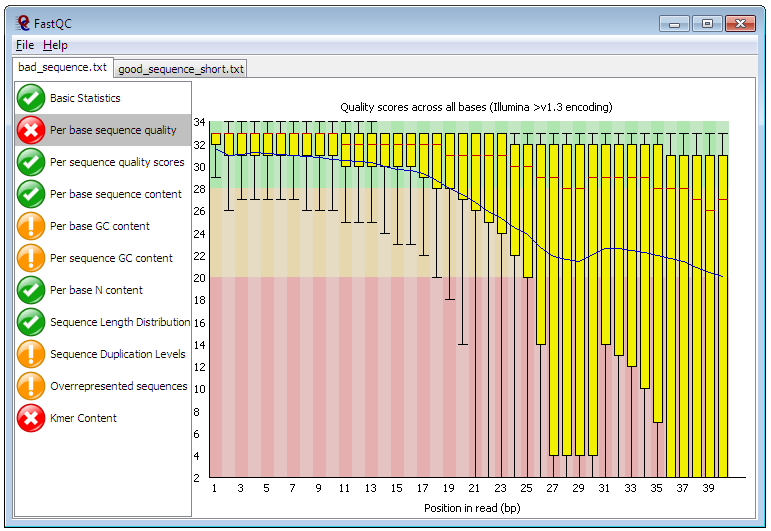
\includegraphics[FastQC]{img/fastqc.png}
\end{center}


\hypertarget{analysis-steps}{%
\subsubsection{Analysis Steps}\label{analysis-steps}}

Bioinformatic processing of data into biologically-meaningful outputs is
often a multi stage process. Just like working in the laboratory, it's
useful to break this process down into individual steps and have a plan
before you start the analysis.

\begin{itemize}
\tightlist
\item
  \textbf{Step 1}. Set up a directory for the QC analysis
\item
  \textbf{Step 2}. Use FastQC to QC the sequence data for each isolate
\item
  \textbf{Step 3}. Gather together all the FastQC reports into a single
  QC report
\item
  \textbf{Step 4}. Run bactinspector on all the isolates to determine
  the species
\item
  \textbf{Step 5}. Assess the QC results and remove any isolates that do
  not pass your QC threshold from further analysis
\item
  \textbf{Step 6}. Summarise your findings (text and screenshots) for
  inclusion in your presentation
\end{itemize}

\hypertarget{software-tools}{%
\subsubsection{Software Tools}\label{software-tools}}

The recommended software to use in this task are:

\begin{itemize}
\tightlist
\item
  FastQC
\item
  MultiQC
\item
  Bactinspector
\end{itemize}

There is a conda environment called \texttt{qc} that contains these
tools. To activate it use:

\texttt{conda\ activate\ qc}

\hypertarget{questions}{%
\subsubsection{Questions}\label{questions}}

The questions you want to ask of the data are:

\begin{itemize}
\tightlist
\item
  What is the yield and sequencing depth for each isolate and is it
  adequate?
\item
  Is the sequencing quality adequate for each of the isolates?
\item
  Are all the isolates the species that you expect?
\end{itemize}

    \hypertarget{task-2-phylogenetic-analysis}{%
\subsection{Task 2: Phylogenetic
analysis}\label{task-2-phylogenetic-analysis}}

In this task you will map the sequence data to the \textit{Salmonella
enterica Typhimurium SL1344} reference genome, call SNPs and build a
phylogenetic tree from the SNP data.

\hypertarget{analysis-steps}{%
\subsubsection{Analysis Steps}\label{analysis-steps}}

A rough guide of the steps involved in this task is below. Check that
you understand the principles of each one and then get started:

\begin{itemize}
\tightlist
\item
  \textbf{Step 1}. Set up a directory for the phylogenetic analysis
\item
  \textbf{Step 2}. Map, call SNPs and create pseudogenomes for each
  isolate
\item
  \textbf{Step 3}. Create a whole genome sequence alignment fusing all
  the pseudogenomes
\item
  \textbf{Step 4}. Identify the SNPs in the pseudogenome alignment
\item
  \textbf{Step 5}. Build a phylogenetic tree
\item
  \textbf{Step 6}. Root the tree
\item
  \textbf{Step 7}. Interpret your phylogeny
\item
  \textbf{Step 8}. Summarise your findings (text and screenshots) for
  inclusion in your presentation
\end{itemize}

    \hypertarget{software-tools}{%
\subsubsection{Software Tools}\label{software-tools}}

The recommended software to use in this task are:

\begin{itemize}
\tightlist
\item
  Bactmap nextflow pipeline
\item
  assembly-stats
\item
  snp-sites
\item
  iqtree
\item
  FigTree
\end{itemize}

The conda environments that contain the required software are
\texttt{nextflow-pipelines} and \texttt{snp-phylogeny}.

\hypertarget{questions}{%
\subsubsection{Questions}\label{questions}}

Look at your phylogenetic tree in Figtree, take some time to make some
general observations:

\begin{itemize}
\tightlist
\item
  Are there distinct clades present in the isolates?
\item
  Are there isolates that do not cluster with other isolates?
\end{itemize}

A picture of your tree as well as your general observations about it
should go into your group presentation. Take some time to make figure(s)
you are happy with and create a PDF picture file by selecting
\texttt{File\ \textgreater{}\ export\ PDF}.


\begin{center}
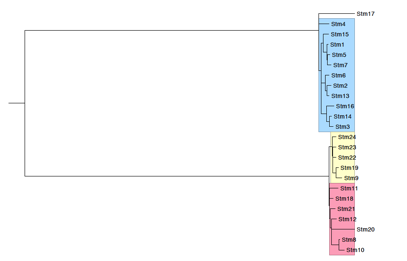
\includegraphics[Phylogenetic tree of isolates]{img/tree.png}
\end{center}


    \hypertarget{task-3-antimicrobial-resistance-screening}{%
\subsection{Task 3: Antimicrobial resistance
screening}\label{task-3-antimicrobial-resistance-screening}}

In this task you will screen your isolates for antimicrobial resistance
(AMR) genes using ARIBA and the CARD database.

\hypertarget{analysis-steps}{%
\subsubsection{Analysis Steps}\label{analysis-steps}}

\begin{itemize}
\tightlist
\item
  \textbf{Step 1.} Set up a directory for the AMR analysis
\item
  \textbf{Step 2.} Download and prepare the CARD database for use with
  ARIBA
\item
  \textbf{Step 3.} Run ARIBA on your isolates
\item
  \textbf{Step 4.} Summarise all the ARIBA results into one report
\item
  \textbf{Step 5.} Visualise the outputs in Phandango
\item
  \textbf{Step 6.} Compare resistance genes found with your phenotypic
  data
\item
  \textbf{Step 7.} Summarise your findings (text and screenshots) for
  inclusion in your presentation
\end{itemize}

\hypertarget{software-tools}{%
\subsubsection{Software Tools}\label{software-tools}}

The recommended software to use in this task are:

\begin{itemize}
\tightlist
\item
  CARD database
\item
  ARIBA
\item
  Phandango
\end{itemize}

The conda environment that contain the required software is
\texttt{ariba-2.14.6}

    \hypertarget{questions}{%
\subsubsection{Questions}\label{questions}}

Open the \texttt{all\_results.summary.phandango.tre} and
\texttt{all\_results.summary.phandango.csv} produced by ARIBA in
Phandago. On the left hand side is a dendogram of the phylogenetic
relationship of the resistance data and the isolates. On the top panel
are the matching resistance genes found. The green colour indicates
positive match and salmon pink is a negative match.


\begin{center}
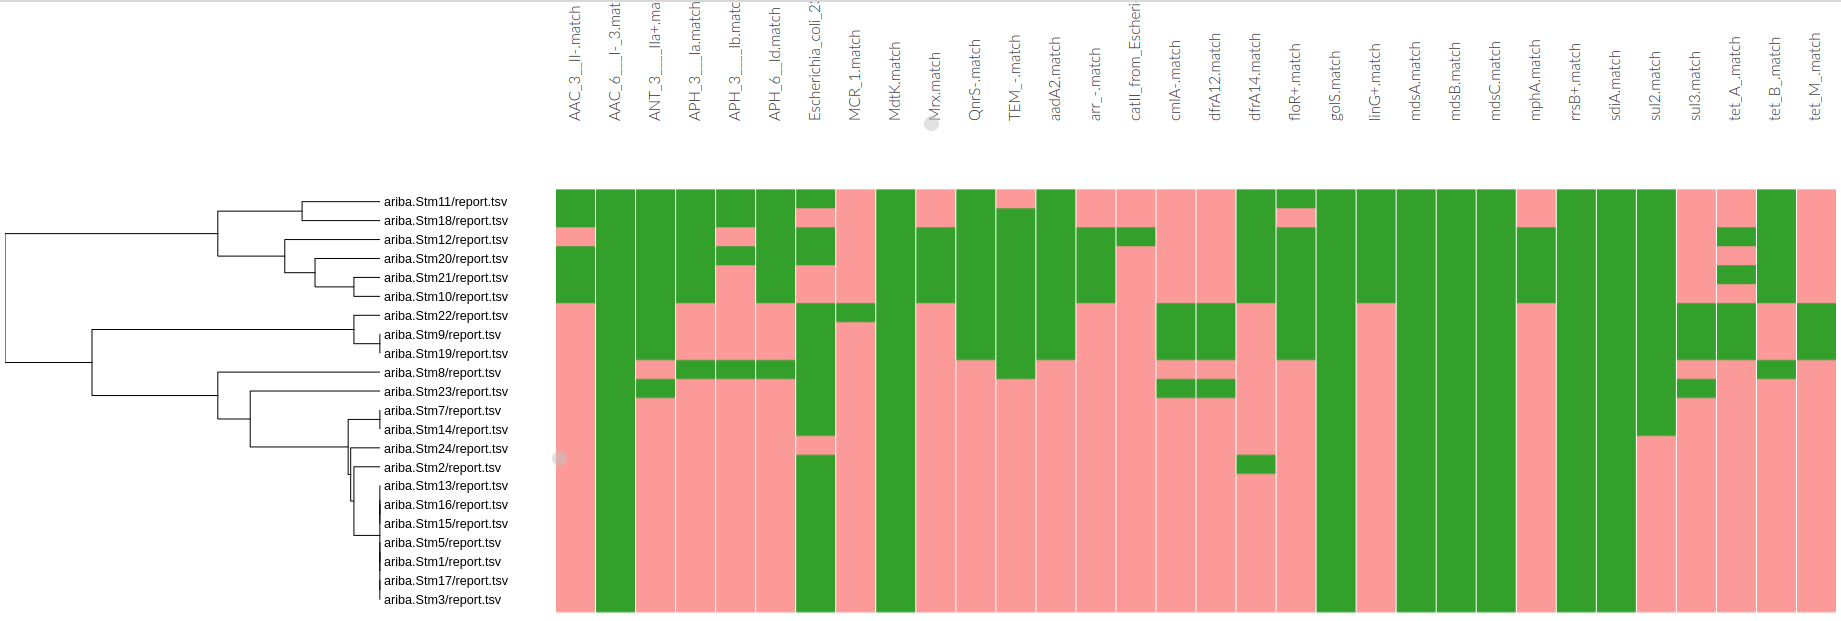
\includegraphics[AMR results in Phandango]{img/phandango.png}
\end{center}


Consult the CARD database for the resistance phenotype of the genes
detected. Note that underscores (\_) in the output data denotes prime
(`) or bracket, therefore AAC\_3\_-II is AAC(3)-II. The codes for these
are in a file named \texttt{01.filter.check\_metadata.tsv} produced when
you prepared your database. Consult the \texttt{report.tsv} of the
particular sample of interest for the gene names. You can open both .tsv
files in excel.

Some general points to consider when summarizing your finding for
antimicrobial resistance (AMR) screen.

\begin{itemize}
\tightlist
\item
  Does the presence of the gene correlate well with the phenotypic
  results?
\item
  Is it the same in multiple isolates that share the resistance?
\end{itemize}

To help you in your discussions, summarized in the table below are the
most frequently observed antimicrobial resistance patterns of S.
Typhimurium strains between 1996 and 2016 taken from Wang et al., 2019
(PMID: 311340204).

Below are genes found in your* isolates that confer resistance to some
of the antibiotics below. Can you match isolates to any of the patterns
listed? Ampicillin (A): aac, aph. Chlorampheniol/Florfenicol (C): cmlA,
floR. Streptmycin (S): aadA2. Sulfonamide (Su): sul2 and sul3.
Tetracycline (T): tet.

*Multiple genes can confer resistance to the same class of
antimicrobials.


\begin{center}
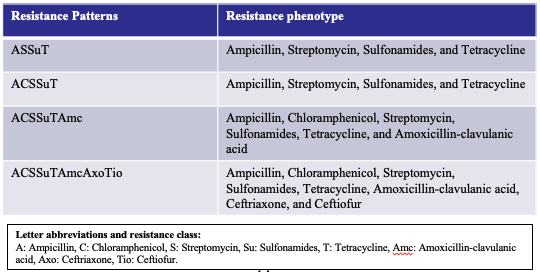
\includegraphics[AMR Resistance Patterns]{img/gene_table.png}
\end{center}


    \hypertarget{task-4-data-visualisation-with-microreact}{%
\subsection{Task 4: Data visualisation with
Microreact}\label{task-4-data-visualisation-with-microreact}}

Use Microreact to visualize and explore your tree and metadata.
Microreact enables you to visualize phylogenetic relationships of
isolates linked to geographic locations. You can also display other
information you find useful and to do so, you need only format your
metadata table. To save time we have prepared a metadata table
compatible with microreact and it is called
\texttt{microreact\_metadata.csv}. It contains latitude and longitude
values for location, date of collection and some selected amr results
from the ARIBA analysis. The different metadata fields have also been
assigned a colour code that will be interpreted by Microreact. Take a
look at this file.


\begin{center}
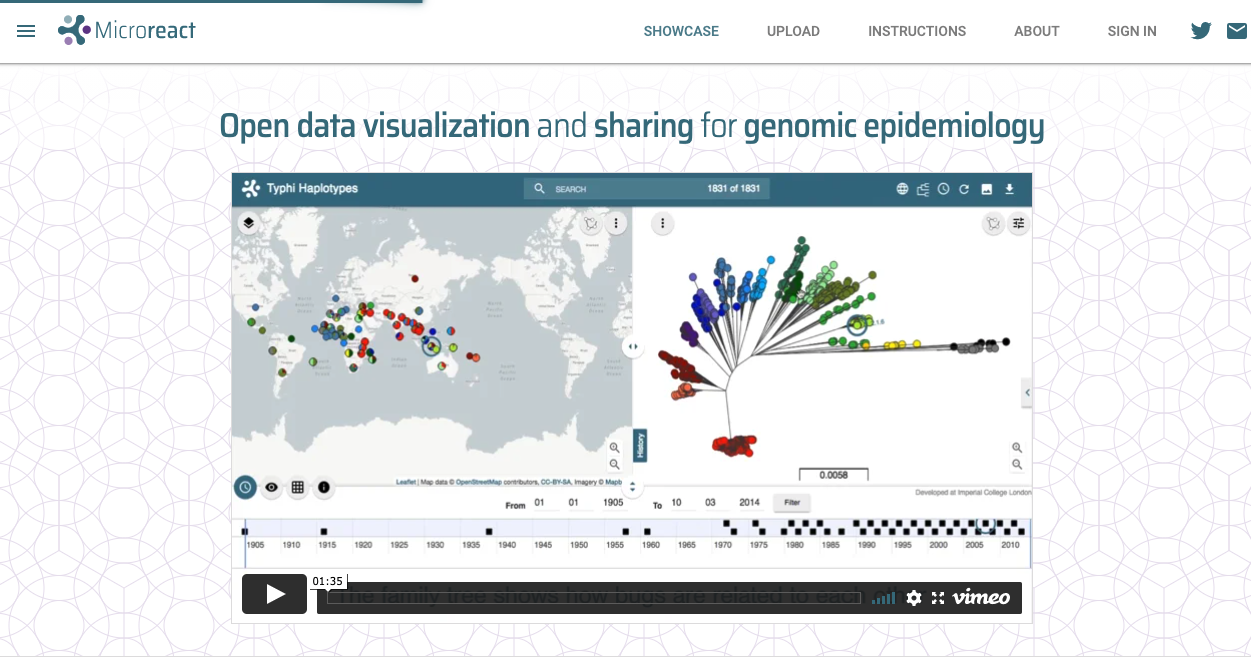
\includegraphics[Microreact]{img/microreact.png}
\end{center}


\hypertarget{location-information}{%
\subsubsection{Location information}\label{location-information}}

There are plenty of ways to generate latitude and longitude coordinates
(e.g.~using a simple search on google) for locations, however with
multiple samples, it is easier to submit this in batches. You can use a
toll called Data-flo, which allows you to paste the name your locations,
returns a list of geographic coordinates. To save time, we have already
generated these coordinates for the locations and included them in the
metadata file.

\hypertarget{creating-a-project-in-microreact}{%
\subsubsection{Creating a project in
Microreact}\label{creating-a-project-in-microreact}}

You will need the NEWICK (.nwk) file from your phylogenetic analysis and
the .csv metadata file mentioned above. Create a new project in
Microreact by dragging and dropping them into the browser on the
Microreact page. Create a map by selecting the edit icon in the right
hand corner and selecting `Create New Map'.


\begin{center}
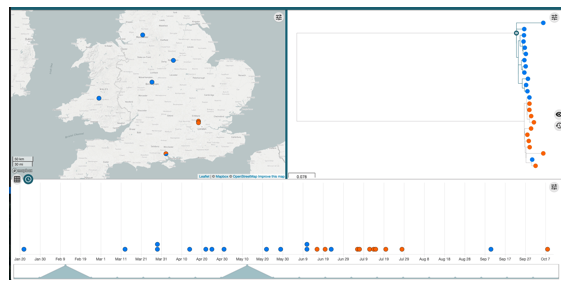
\includegraphics[Data in microreact]{img/microreact-data.png}
\end{center}


The resulting map and tree enables you to query your data. Notice we
have assigned colour to the samples resistant or sensitive to
aminoglycosides encoded by aadA2, but you can choose to group the
samples however you want. For example, you can include other
antimicrobial resistance information. All you will have to do is add the
resistance gene data from the ariba results.

    \hypertarget{task-5-summarise-your-findings-for-the-presentation}{%
\subsection{Task 5: Summarise your findings for the
presentation}\label{task-5-summarise-your-findings-for-the-presentation}}

Create a short 5 mins presentation summarising your findings. A
suggested outline for the presemtations is:

\begin{itemize}
\tightlist
\item
  Title slide (include your group name and individual names)
\item
  Aims of the project
\item
  Summary of the data
\item
  Methods for each task (how you analysed your data)
\item
  Results from each task (use lots of screenshots!)
\item
  Findings and conclusions
\end{itemize}

Some things to consider when you are interpreting your results, look at
the distribution of your isolates across the country when coloured by:

\hypertarget{clade}{%
\subsubsection{Clade}\label{clade}}

\begin{itemize}
\tightlist
\item
  How many clades are there?
\item
  How are the isolates distributed?
\item
  Are there any patterns you can see to the distribution?
\item
  What factors might be driving the distribution?
\end{itemize}

\hypertarget{antimicrobial-resistances}{%
\subsubsection{Antimicrobial
resistances}\label{antimicrobial-resistances}}

\begin{itemize}
\tightlist
\item
  Are there patterns to any of the resistances?
\item
  And is this related to clades?
\item
  Are there any genes that confer resistance to antimicrobials used to
  treat Salmonella cases?
\end{itemize}

Decide among the group who will present each slide, if possible we would
like to see everyone from the group present at least one slide each.

    \textbf{DISCLAIMER:} All the locations and dates of the Salmonella
isolates are fictitious and solely for educational purposes.


    % Add a bibliography block to the postdoc



\end{document}
